\section{Fase di Test}
Tutte le pagine e il relativo codice sono stati sottoposti a una validazione attraverso i seguenti strumenti:
    \begin{itemize}
        \item Validatore online W3C per il CSS \url{https://jigsaw.w3.org/css-validator/};
        \item Validatore online W3C per l'HTML \url{https://validator.w3.org/};
        \item Contrast Analyzer per verificare che i colori usati \url{https://webaim.org/resources/contrastchecker/}.
    \end{itemize}
    La validazione del codice HTML è stata fatta incollando direttamente il codice sorgente prodotto dalle pagine PHP nel validatore W3C, in modo tale da poter validare tutto quel codice non presente nelle pagine in HTML.
    Il sito è stato inoltre testato sui seguenti browser:
    \begin{itemize}
        \item Safari;
        \item Microsoft Internet Explorer/Edge;
        \item Microsoft Edge (beta) basato su Chromium;
        \item Google Chrome;
        \item Mozilla Firefox.
    \end{itemize}
        \subsection{Mobile}
        Il sito è stato testato su dispositivi Android e iOS e presenta layout o comportamenti differenti (ad esempio le select) per cause che dipendono dal sistema operativo. Abbiamo cercato di renderlo il più utilizzabile possibile, tuttavia l'area amministratore presenta un layout che non si adattava alla visualizzazione su schermi di piccole dimensioni come quelle degli smartphone. Riteniamo che le operazioni svolte da un amministratore siano svolte solamente attraverso dispositivi desktop o tablet di dimensioni sufficientemente grandi e per questo motivo l'area amministratore non è del tutto accessibile su smartphone.

	\subsection{Eccezioni}
	La validazione del codice HTML della pagina animali con lo standard definito da XHTML 1.0 - Strict ha prodotto l'errore in figura a causa del fatto che l'attributo "placeholder" per il tag $<$input$>$ è stato introdotto con HTML 5.\\
	
	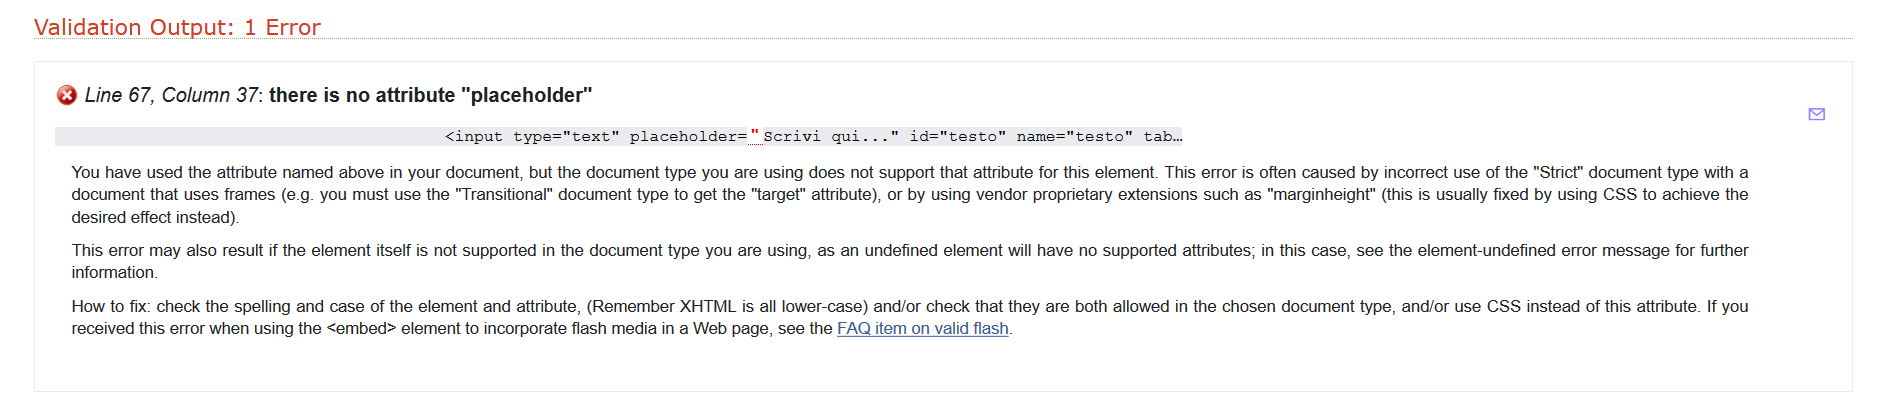
\includegraphics[width=35pc]{./img/erroreValidazione.png}
	\captionof{figure}{Errore di validazione dell'attributo "placeholder"}
	
	La scelta di mantenere l'attributo "placeholder" al tag $<$input$>$ nonostante l'errore di validazione è stata discussa e approvata in quanto i browser più diffusi, e su cui è anche stato testato il sito, interpretano correttamente il tag e l'attributo in discussione.
\pagebreak